\xchapter{Evaluation}{}
\label{sec:evaluation}
\acresetall

In this chapter we present the results of a series of experiments to evaluate the approximation algorithm and SIM in relation to the 
maximum out-degree and the costs of the paths from the source node to each terminal in the generated arborescence. 
We first describe the parameters used in the experiments and implementation details (Section \ref{sec:parameters}). 
Then, we describe the algorithms and metrics 
used in the experiments (Section \ref{sec:metrics}). At last, we present the results of experiments for the chosen metrics and algorithms (Section \ref{sec:experiment_results}).

As mentioned before, we were not able to satisfy the spanner constraint. However, our experiments show quite good results. 
More specifically, for the approximation algorithm, in more than half of the situations there was no violation of the spanner constraint (this will be better 
explained in Section \ref{sec:experiment_results}, through graphics) and in the other half the violation was by a low factor (on average, less than 10\%). 
For the heuristic, although the results were not as good as for the other algorithm, the ratio of violation (which is the main metric) was quite low too, 
and the heuristic always outperformed the other algorithms concerning the degree, besides showing a uniform behaviour for both the degree and spanner violation, 
what contributes to scalability.
%Then, we analyse the results of simulations for the proposed algorithms and 
%for a simple algorithm by comparing the maximum out-degree and paths' final costs of the resulted topologies (Section \ref{sec:degree_path-costs}).

\section{Parameters and Implementation Details}
\label{sec:parameters}
We created a specific Java program to perform the experiments. The source code of the program can be found in \cite{DSMDStPLink2012}. 

In all experiment scenarios, nodes were spread in a 500$\times$500 Euclidian space. 
For each node $u$ we assumed a transmission range of approximately 125 distance units. 
Each node can communicate with all nodes inside the circumference with radius equal to its range and centered at that node.
The cost associated with each edge $(u, v)$ is equal to the Euclidean distance between $u$ and $v$.

The number of nodes (\emph{network size}), $n$, ranged from 60 to 300. For each network size, the number of terminals, $t$, ranged from 10 to 50. 
For each pair of network size and terminals set size,
% $\langle n_i,t_j\rangle$, 
we performed experiments with different spanning factors, $sf$, ranging from 1 to 2. 
For each combination of network size, terminals set size and spanning factor,
%$<n_i,t_j,sf_z>$, 
we generated 30 scenarios. 

The algorithm for solving the MSC problem is based on an algorithm described in \cite{Chekuri2004}. This algorithm is based
on an \emph{$\alpha$-approximate oracle}, which results a solution set whose quality deviates by a bounded factor from an optimum set (see Section \ref{sec:solve_msc} for more details). 
We implemented an optimum oracle, i.e. an $1$-approximate oracle.

%falar da distanccia maxima assumida e da funcao de custo assumida (distancia euclideana) -> nao pode dar problema esta suposicao ?.
%falar do oracle
%falar dos parametros da rede

\section{Algorithms and Metrics}
\label{sec:metrics}
As we are not aware of any other algorithm to \mbox{DSMDStP}, we compared the algorithms we presented in this dissertation 
against a shortest path tree algorithm (SPT), i.e. an algorithm that calculates a tree formed by shortest paths from the source node to each
of the terminals. The reason for choosing SPT is that it is a simple and efficient algorithm that generates a tree which satisfies the
spanner restrictions as it generates a single-sink 1-spanner Steiner tree ($k=1$). 
Another reason for choosing SPT were the similarities between the proposed algorithms (mainly the approximation algorithm) 
and SPT, since the criterion for choosing the spanner paths (paths that respect the spanner property) is based on shortest paths. These similarities were 
reflected in the experiment results.

We used four metrics to compare and analyze the algorithms. For each metric, we considered the average of the 30 scenarios. Besides evaluating the maximum out-degree, 
we measured the final path costs. As we cannot guarantee a root-stretch factor of $k$, but one of $k \cdot \left(1 + \frac{max_{t\in T}\{dist(s,t,G)\}}{min_{t \in T}\{dist(s,t,G)\}}\right)$ and $k \cdot (\lfloor\sqrt{|T|}\rfloor + 2)$ 
for Algorithm \ref{alg:approximation} and SIM respectively, we calculated the ratio between the final path's cost and the desired path's cost 
(i.e. $k$ times the shortest cost path from the source node to the terminal). We would like to verify the extent of the violation in the experiments. 
Let us 
call this ratio \emph{Cost Violation Ratio} (CVR). 
CVR was calculated using the following formula:
%\footnote{Flavio, provavelmente a metrica correta deveria ser $\frac{\sum_{\forall t \in T}\frac{dist(s,t,\mathcal{A}_f)}{k \cdot dist(s,t,G)}}{|T|}$. Como a simulacao 
%demora, nao quis rever isso AGORA. Mas, acredito eu que os valores das duas metricas devam ser similares. Entao eh possivel adiantar a analise}:

\begin{equation}
\label{eq:cost_violation_ratio}
%  CVR = \frac{\sum_{\forall t \in T}dist(s,t,\mathcal{A}_f)}{\sum_{\forall t \in T}k \cdot dist(s,t,G)}.
  CVR = \frac{\sum_{\forall t \in T_{vio}}\frac{dist(s,t,\mathcal{A}_f)}{k \cdot dist(s,t,G)}}{|T_{vio}|}
\end{equation}

where: %\linebreak
\begin{center}
 $T_{vio} \subseteq T = \lbrace t | t \in T \wedge dist(s,t,\mathcal{A}_f) > k \cdot dist(s,t,G) \rbrace$. 
\end{center}

Observe that we take into consideration only the terminals whose final costs violate the spanner constraint 
(represented by the set $T_{vio}$). We defined the metric in this way because we would like to answer the following question: when the violation occurs, by how much does it occur? 
Even though this metric worse our results
%\footnote{We could then model CVR in an alternative way, e.g., $CVR = \frac{\sum_{\forall t \in T}max\lbrace 1, \frac{dist(s,t,\mathcal{A}_f)}{k \cdot dist(s,t,G)} \rbrace}{|T|}$. 
%where $R(t)$ holds 1 if $\frac{dist(s,t,\mathcal{A}_f)}{k \cdot dist(s,t,G)} \leq 1$, or $\frac{dist(s,t,\mathcal{A}_f)}{k \cdot dist(s,t,G)}$ otherwise
%But, CVR would then merge two different concepts: the violation ratio itself and the percentage of violated terminals} 
(by increasing the CVR value), it is a more accurate metric for the former question than we had considered all the terminals. CVR's value is always 
$\ge 1$. The lower the CVR, the lower the violation. 
%Since we average CVR by the number of generated scenarios, and in order to capture the worst violation ratio's value, 

As CVR is an average, we also calculated the worst violation ratio (the greatest ratio in the numerator of CVR). Let us call it \emph{MAX\_CVR}. 
Although we ran 30 scenarios for each pair of network size and terminals set size, in order to keep the coherency of the metrics, we averaged CVR and MAX\_CVR only by the number of scenarios where violation occurred. 
%So, we also thought convenient to calculate the percentage of violated scenarios. 

The paths to the nodes covered in the first phase of our algorithm and in the first iteration of SIM have their spanner constraints
satisfied. It is supposed, however, that more terminals have their spanner constraints satisfied, as we use the criteria 
of choosing shortest cost paths in the algorithms. 
As in CVR's denominator we considered $|T_{vio}|$ instead of $|T|$, 
we calculated additionally the percentage of spanner constraints violated. 
This percentage is represented by the PVT (Percentage of Violated Terminals) metric. 
%We call this percentage by \emph{Percentage of Violated Terminals} (PVT). 
Similar to CVR, we averaged PVT by the number of scenarios where violation occurred. 
Formally: 

\begin{equation}
\label{eq:percentage_violated_terminals}
%  CVR = \frac{\sum_{\forall t \in T}dist(s,t,\mathcal{A}_f)}{\sum_{\forall t \in T}k \cdot dist(s,t,G)}.
  PVT = \frac{|T_{vio}|}{|T|} \cdot 100 \%.
\end{equation}

For both CVR and PVT, we considered only the scenarios where violation occurred. 
We calculated additionally the percentage of scenarios where violation occurred. This is represented by the PVR (Percentage of Violated Runs)
metric.

%As mentioned in Section \ref{sec:complete_algorithm}, the terminals covered in the first phase of Algorithm \ref{alg:approximation} have their 
%spanner constraint satisfied. So, in order to quantify this characteristic of the algorithm, we measured the percentage of terminals that have their 
%spanner constraint theoretically satisfied, i.e., the percentage of terminals covered in the first phase of Algorithm \ref{alg:approximation}.

\section{Experiment Results}
\label{sec:experiment_results}
Figure \ref{fig:degree_abscissae} shows the maximum out-degree for three different parameters: network size (Figure \ref{fig:degree_abscissae}a), 
size of the terminals set (Figure \ref{fig:degree_abscissae}b) and spanning factor (Figure \ref{fig:degree_abscissae}c). 
For each of these parameters, fixed values for the others were used. The fixed values are indicated by the labels above the plots 
(\emph{NS} - Network Size; \emph{Ter} - Terminals Set Size; 
\emph{SF} - Spanning Factor). Algorithm \ref{alg:approximation} is referred throughout this section by the abbreviation \emph{APPROX}.

In Figure \ref{fig:degree_abscissae}a, generally, the degree value is stable for both APPROX and SIM, 
irrespective of the network size. So, regarding the degree, these algorithms support network scalability well. 
On the other hand, the degree of SPT increases quickly and the final arborescence has a degree three times greater than the other algorithms in denser networks. 
Regarding the number of terminals (Figure \ref{fig:degree_abscissae}b), the greater the number of terminals, the greater the degree of the three algorithms. This behaviour is expected by the 
two proposed algorithms, since in each step (each \emph{phase} for APPROX and each \emph{iteration} for SIM) of the algorithms, the possible maximum 
degree is affected by the number of terminals. But, the difference between the three algorithms is the slope ratio. For the proposed algorithms the 
increasing ratio is low whereas it is high for SPT. Finally, in Figure \ref{fig:degree_abscissae}c, we ranged the spanning factor. As expected, 
the degree resulted from applying SPT is the same, besides being high. For the lowest value of the spanning factor,
APPROX yielded a much higher degree when comparing to the cases with higher spanning factors,
but the maximum degree decreases drastically with the increase in the spanning factor.
SIM exhibits a uniform behaviour, so the achieved maximum degree mean was roughly unaffected by the spanning factor. For all the three parameters, SIM outperformed APPROX.
\begin{figure*}[!th]
\centering
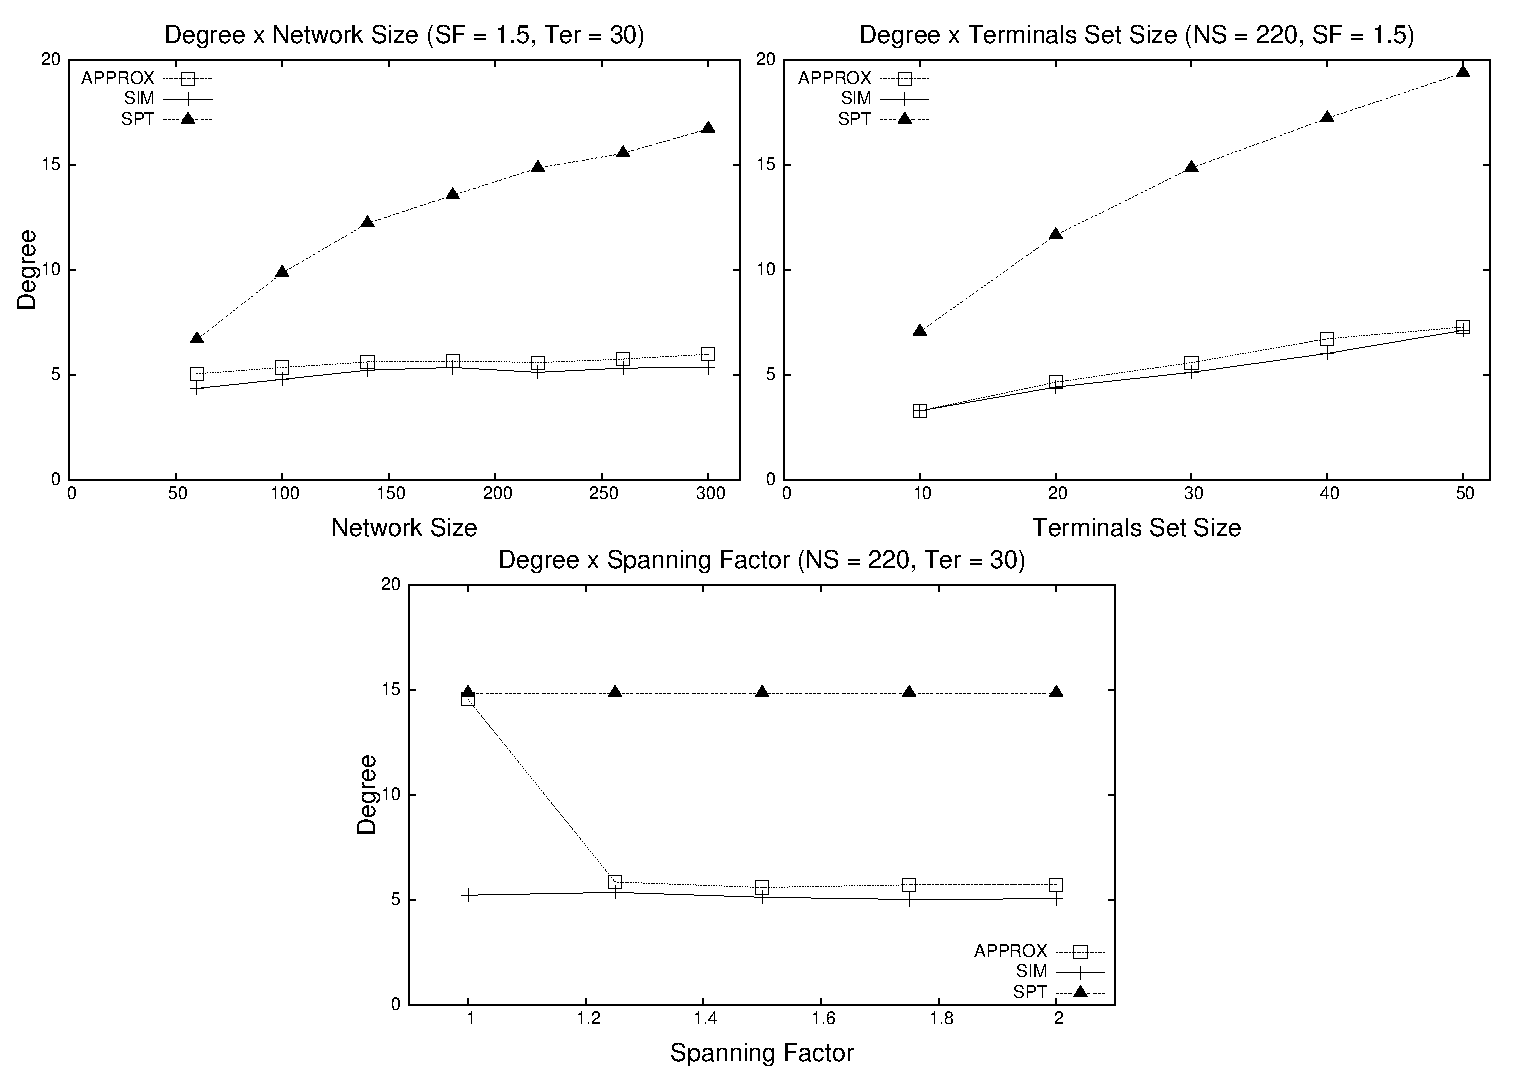
\includegraphics[scale=0.63]{imagens/grau-220-3_graficos_nao_alinhados}
\caption{Maximum out-degree in function of (a) network size, (b) number of terminals, and (c) spanning factor}
\label{fig:degree_abscissae}
\end{figure*}
\begin{figure}[!th]
\centering
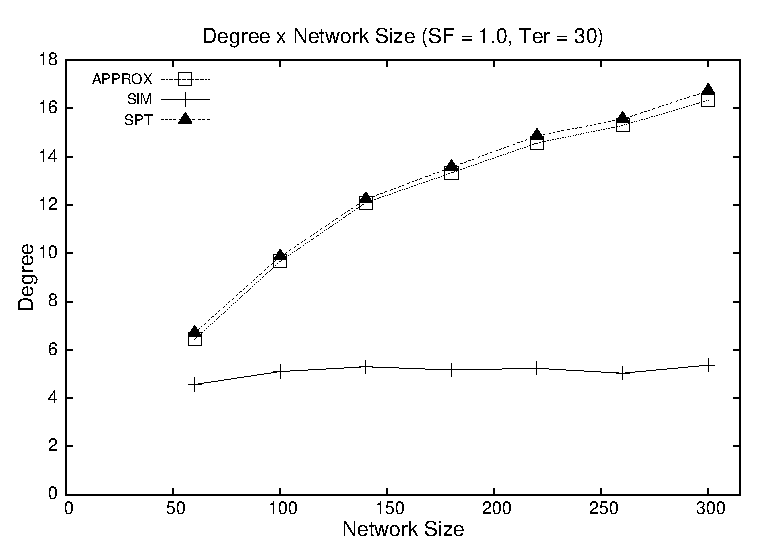
\includegraphics[scale=0.63]{imagens/grau-220-sp1}
\caption{Degree x Network Size when spanning factor is 1}
\label{fig:degree_network-size}
\end{figure}
\begin{figure*}[!th]
\centering
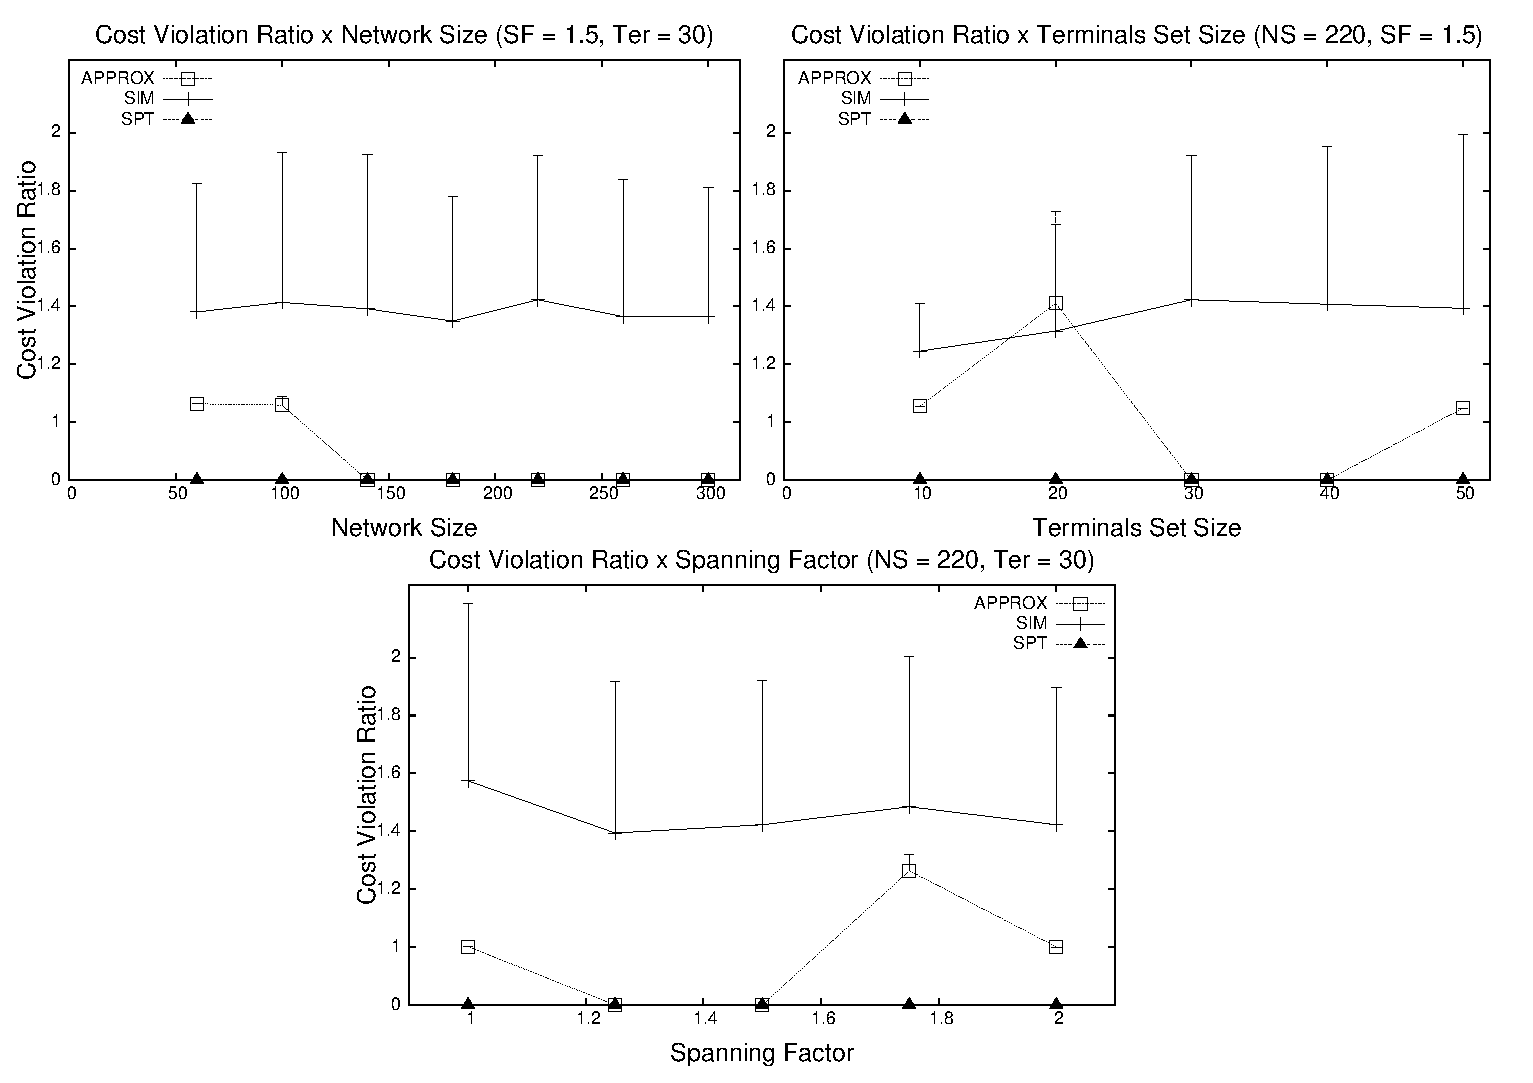
\includegraphics[scale=0.63]{imagens/violatedTerminalsCVR-220-3_graficos_nao_alinhados}
\caption{Cost Violation Ratio in function of (a) network size, (b) number of terminals, and (c) spanning factor}
\label{fig:cvr_abscissae}
\end{figure*}
\begin{figure*}[!th]
\centering
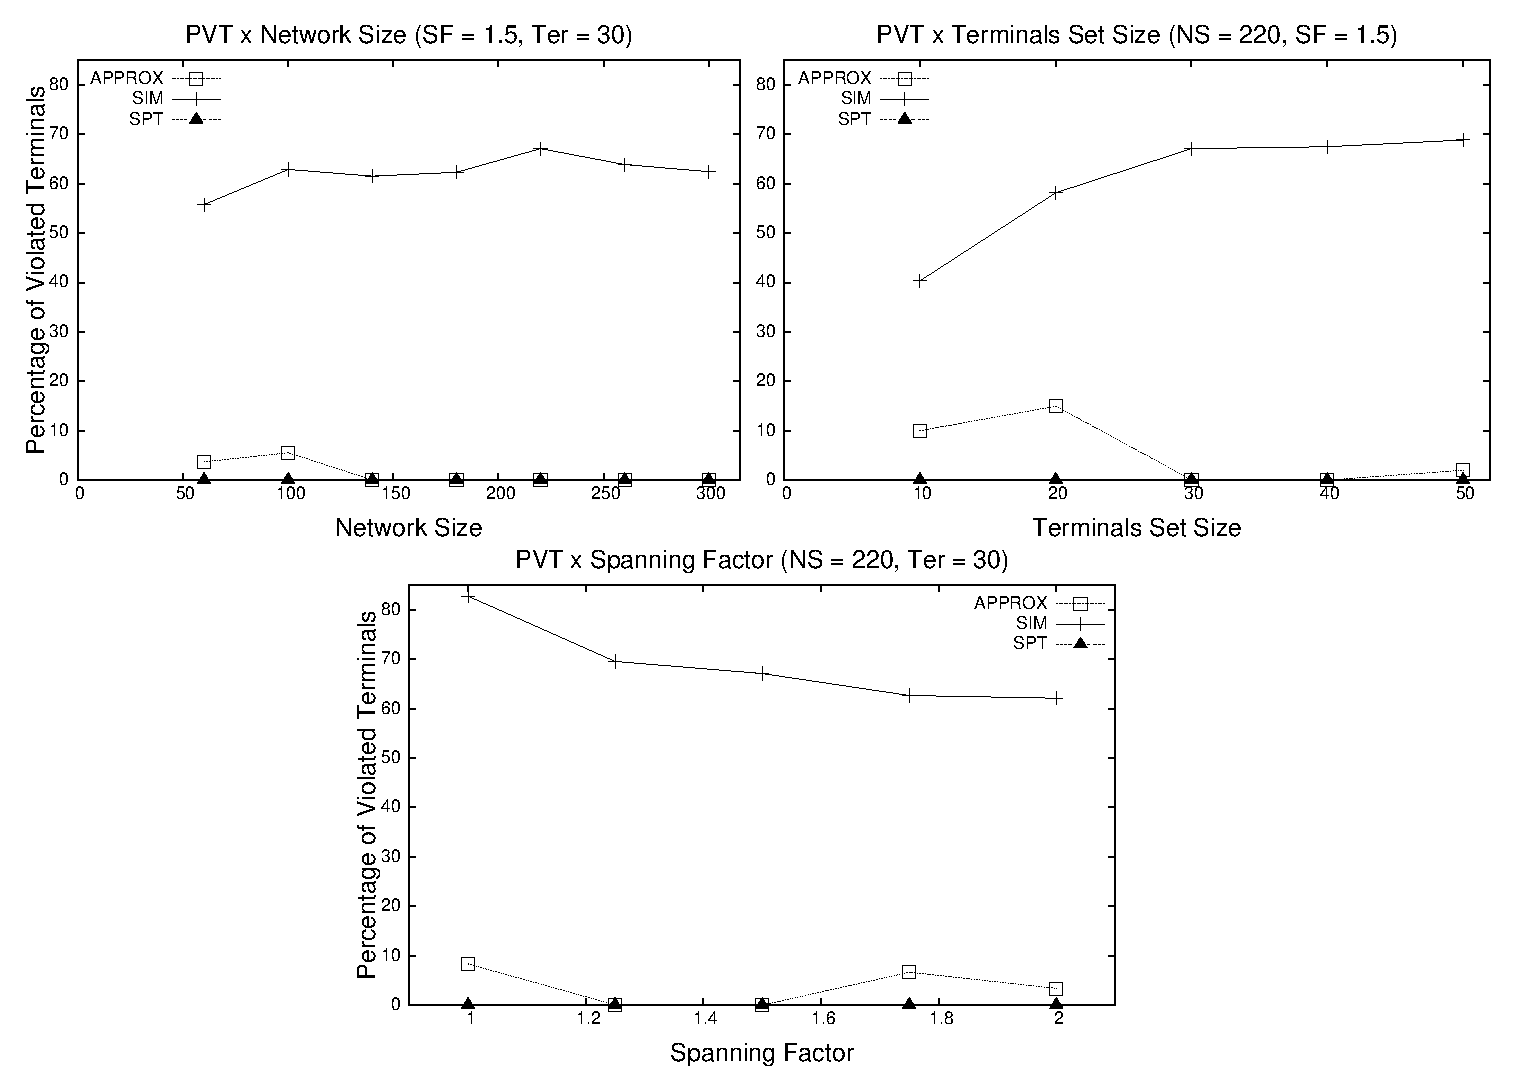
\includegraphics[scale=0.63]{imagens/violatedNodesRatio-220-3_graficos_nao_alinhados}
\caption{Percentage of Violated Terminals in function of (a) network size, (b) number of terminals, and (c) spanning factor}
\label{fig:violated-terminals_abscissae}
\end{figure*}

%Figure \ref{fig:degree_abscissae}c gives us a clue that Algorithm \ref{alg:approximation} suffers a lot when the spanning factor is restrictive. Moreover, 
Since APPROX imitates, in some aspects, the SPT algorithm, we evaluated the algorithms for the specific case of 
spanning factor equal to $1$. 
This graphic is illustrated by Figure \ref{fig:degree_network-size}. Observe that the curve of APPROX  
is very close to the curve of SPT. 
Assuming a spanning factor of 1 corresponds to the situation when the restrictions on the paths from the source node to
the terminals correspond to the minimum cost paths.
As the restrictions are tighter, there will be less paths to choose
%(actually, in the majority of cases it will be only one and the set of paths will correspond to subpaths of a SPT to these terminals) 
leading to the uncovered terminals and respecting the constraints in the second phase of APPROX. This might contribute
to an increase in the degree of nodes. 
%and Algorithm \ref{alg:approximation} tries to do this. This is worsen by the fact that, in the second phase, there will be only very few paths 
%(actually, in the majority it will be only one) leading to the uncovered terminals and respecting the constraints imposed by the modeling of the edges of MSC. 
%So, not only there will be very few available paths to the terminals in the second phase but also the majority of terminals will be in this situation 
%(in part, illustrated by Figure \ref{fig:violated-terminals_abscissae}c), making APPROX behave similarly to SPT. 
On the other hand, SIM is quite good for scalability in this situation too. 
Although both APPROX and SIM apply the algorithm for the MSC problem, only APPROX exhibited behaviour similar to SPT. This might be explained by the restrictions 
on the edges that are allowed to be part of a MSC instance, where for APPROX the restriction considers paths from the source node to the terminal and for SIM the restriction only considers 
the path from a covered node (which is unique) to the terminal. 

%This is corroborated by the low percentage of terminals covered in first phase of the algorithm, showed in Figure \ref{fig:ter_covered} 
%(to be presented later). Due to what was stated before, the number of nodes covered in first phase was low. So, 

Figure \ref{fig:cvr_abscissae} shows the cost violation ratio (CVR) for the three different parameters
(network size, terminals set size and spanning factor). The vertical bars on each point were used to represent MAX\_CVR
(the top of the bars represents its value). On the $y$ axis, the value 0 indicates that at that point no violation for any terminal occurred. 
%the label \emph{N/V} is an acronym for \emph{Not Violated}, which means in that point no violation for any terminal occurred. 
For this metric, it is obvious that SPT will always exhibit the best behaviour (all of its points are on the line $y = 0$), 
as it finds shortest paths. The closer the value to 1, the lesser the violation. 
In Figure \ref{fig:cvr_abscissae}a, the CVR's value for APPROX is quite close to 1 for the first 2 points, 
and no violation occurs for the others. 
The CVR's value for SIM is greater than APPROX, but it is still low (1.4 in average) and it is uniform. In Figures \ref{fig:cvr_abscissae}b and \ref{fig:cvr_abscissae}c, 
the CVR's behaviour is similar to the one presented in Figure \ref{fig:cvr_abscissae}a for both proposed algorithms. Considering APPROX's values, 
in almost half of its abscissa's values no violation occurs and in the other points the CVR's value is close to 1 (except for one point in each graphic). 
Regarding SIM's values, the CVR is again low (between 1.4 and 1.5 in average) and uniform. In the graphics, the behaviour of MAX\_CVR for the algorithms is repeated. 
Regarding the APPROX algorithm, MAX\_CVR is really close to CVR (except for one point in Figure \ref{fig:cvr_abscissae}b) and, in some cases, they are 
almost the same, which it is good because APPROX's worst case is close to the average case. Concerning SIM, the MAX\_CVR is slightly 
higher than CVR, but it is in almost all situations $\le 2$, which is quite acceptable.

CVR measures the quality of violation, but it is important to calculate the amount of violation. PVT 
captures this concept. More specifically, PVT answers the question: when violation occurs, how many terminals violate their constraint? 
The values of PVT are shown in Figure \ref{fig:violated-terminals_abscissae}. 
%Although plotting SPT is unnecessary, we plotted it in order to take its curve as base (mainly for APPROX). 
For all three graphics, the PVT's value is 0 for the same points where no violation 
occurs in Figure \ref{fig:cvr_abscissae}. In Figure \ref{fig:violated-terminals_abscissae}a, the PVT's value for APPROX is quite low (less than 10\%). In fact, 
the behaviour of PVT for APPROX is similar for all the three graphics, where the value exhibited is generally less than 10\%. Concerning SIM, the PVT's value 
is high but it is uniform for the network size (between 60\% and 70\%). 
For SIM, there is a tendency to increase the PVT value with the increse in the terminals set size.
On the other hand, when we vary the spanning factor, the higher the spanning factor, the lower the PVT's value for SIM.

Finally, we evaluated the percentage of scenarios where (at least one) violation occurs (PVR). 
The graphic of PVR is represented by Figure \ref{fig:violated-runs_network-size}. For APPROX, the 
denser the network, the lower PVR is. Additionally, the percentage is no greater than 30\%. Even though this value could be considered, in some senses, to be not  
so low, recall that PVR disregards the percentage of terminals which violate the spanner constraint 
(the run is considered violated even if the constraint is violated for a single terminal) and the amount of violation. The latter is captured by the CVR metric. A variation of the former is captured by PVT metric.
For SIM, PVR has the highest possible value.

\begin{figure}[!th]
\centering
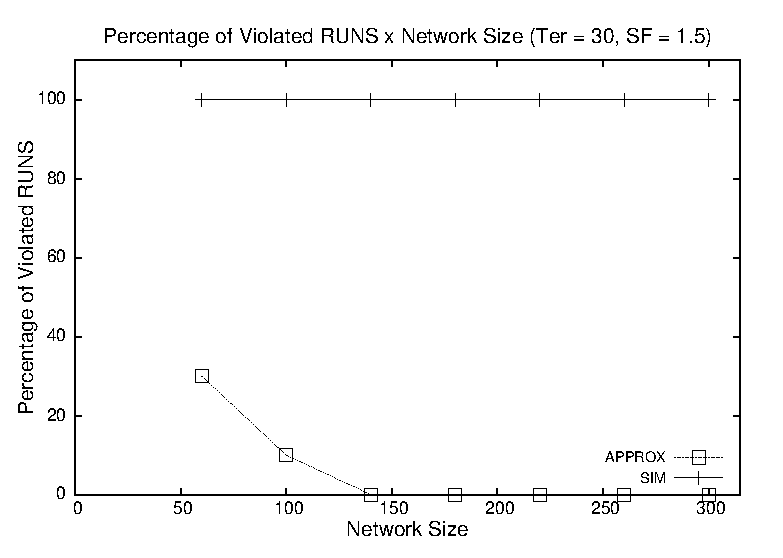
\includegraphics[scale=0.63]{imagens/percViolatedRUNS-ter30sf15}
\caption{Percentage of Violated RUNS x Network Size}
\label{fig:violated-runs_network-size}
\end{figure}

According to our experiments, the maximum out-degree for the proposed algorithms was quite low, except for APPROX in the 
worst scenario when the spanning factor was set to 1 (Figure \ref{fig:degree_abscissae}c). In this scenario, APPROX mimicked SPT's behaviour. 
SIM had uniform behaviour at large, supporting better scalability, and always outperformed APPROX 
in the degree metric. On the other hand, APPROX always outperformed SIM for the CVR, PVT and PVR metrics. More than that, APPROX 
presented very good results for both the quality (CVR) and the quantity (PVT and PVR) of violation. In almost half of abscissa's values (in some situations, more than half) 
no violation occurred. Regarding the quality of violation, when it occurred, the violation was quite low, even in worst cases. The same happened for the 
quantity of violation in the case of APPROX. Considering SIM, although the values were not as so good as for APPROX, 
especially for the quantity metrics, SIM presented very good results for the metric that measures the quality of violation, which is the one that best summarizes 
the analysis of the spanner property. For the CVR metric, the value was quite low (in average 1.4) and even in the worst case it was low (in most cases limited by 2). Furthermore, the values achieved by CVR exhibited an uniform behaviour in general.

%In the next chapter, we are going to conclude the thesis and present future work.
In the next chapter, we discuss extensively the related work, presenting the main results. Moreover, we argue why DSMDStP is 
a new problem, giving the differences between our problem and the related ones.

%In the next chapter, we are going to describe how we could improve the degree guarantee for APPROX through a new modeling of MCG. This new modeling 
%is based on the concepts of \emph{submodular function} and \emph{matroid}. This improvement would be possible due to the results presented in \cite{Calinescu2011}, 
%but doing this we would turn our algorithm into a randomized one.
